\documentclass[../Lael_John_MasterThesis_Draft.tex]{subfiles}
\graphicspath{\subfix[../images]}
\begin{document}
\section{Background to the Counterexample}\label{section:historyconstructions}
In spite of all of these preliminary results indicating positive answers towards Comon's Conjecture, Yaroslav Shitov seemed to arrive at a method of constructing a potential counterexample, as early as 2018 \cite{shitov_counterexample_2018}. An error found in this paper led to the invalidation [REPLACE THIS WORD] of this specific counterexample in 2024, but the period of six years in the interim led to multiple other preprints from Shitov \cites{shitov_comons_2020,shitov_higher_2024,shitov_higher_2024-1}. 

These preprints started with a newer, alternative methodology for the construction of counterexamples. While there is now no material carrying the stamp of peer-review and Shitov's name, his initial contribution and subsequent preprints seem to indicate a viable approach to constructing a counterexample to Comon's conjecture over $\reals$, if not $\complex$. [VALUED TENSORS RATHER THAN FIELD]  

\subsection{Shitov's First Paper in 2018}\label{section:shitovpaper}
The 2018 paper began with taking the ground field as $\complex$, and fixing the notation to be used. The main objects of interest in the paper were order-$3$ tensors, and the introductory section of the paper highlighted the behaviour of such tensors under elementary transformations with respect to their constituent order-$2$ "slices". The construction of the counterexample began with the description of a $100 \times 100$ matrix, partitioned into 20 submatrices [INCLUDE GRAPHIC ILLUSTRATING THIS]. Each submatrix was then mapped to a corresponding $100 \times 100$ matrix, now with entries having the same indices as the submatrix set to $1$ and all other entries as $0$. Taking the $1-$ and $2-$ supports of each of these, and pre- and post-multiplying them with a column-shift operator with parameter $a$ led to another set of matrices of the same size (still $100 \times 100$).

It is at this point that the paper made a concerning [CHANGE WORD?] construction. A set $\mathcal{B}$ was constructed consisting of matrices of distinct formats (viz. $200 \times 200$ and $400 \times 400$). While there is no issue in defining such a set, the paper then constructed "the $\complex$-linear span" of the elements of this set. Addition of quantities that do not live in the same dimensional vector space, without a specified or implied embedding map (at least from this author's knowledge) presented a major problem with following this paper.

Later in the paper a tensor decomposition was described (Eq. 5.6 in \cite{shitov_counterexample_2018}.) This statement was the subject of the erratum published in 2024 \cite{draisma_erratum_2024}. The erratum indicated such a statement was true only in specific cases, but could not be said to hold in general otherwise without proof. Proving the statement has been a non-trivial challenge, and since no answer has been arrived at, the current consensus is that the paper \cite{shitov_counterexample_2018} does not lead to a valid counterexample. [PARAGRAPH IS CLUNKY, TRY REWRITING]

 While certain choices were made during this process that led to unanswered questions, the overall tools for later establishing a valid counterexample were first laid out in this paper. These included the two minor operations - slicing and flattening, and the three major operations - adjoining slices to tensors, generating linear families modulo slices and cloning.


\subsection{Shitov's Subsequent Preprints}\label{section:shitovpreprints}

In the following years, the preprints \cites{shitov_comons_2020,shitov_higher_2024,shitov_higher_2024-1} from Shitov either tackled Comon's conjecture in a restricted setting, or developed tools to construct more general counterexamples. These might also be used to construct a counterexample to Strassen's conjecture (another tensor rank conjecture concerning the additivity of rank). The preprint from 2020 \cite{shitov_comons_2020} tackled the conjecture over $\reals$ and it was this preprint that formed the basis for the paper from Wang and Seigal \cite{wang_lower_2023}.

The constructions made in each preprint followed the same pattern, indicating a common toolset and structure of approach. Each approach saw an order-$d$ tensor as composed of lower order-$(d-1)$ tensors, which allowed for tensors to be transformed by "slice" along a specified mode. Viewing tensors in this manner opened a way to describe tensors modulo these slices --- a useful operation, [seen in both number theory when working with integers modulo primes, and algebraic geometry as a tool to study problems in a more localised setting]. Such a family, when generated, gave an idea of the general properties of the orginal tensor (how many linearly independent slices along a specified mode, maximum slice rank along each mode etc.) Flattenings assisted with the computation of rank for these slices (because computing the rank of matrices is a known and easier problem to solve than doing so for higher order tensors) and the flattenings lent themselves well to describing rank information that might change in the relationship between a tensor and its slices.

These tools allowed for an analysis of any particular tensor, but the construction aspect of this approach became evident with the adjoining of slices to a tensor and the cloning operation. The former operation changed the format of the original tensor with respect to certain chosen slices, and allowed the rank information of the family generated modulo the slices to be preserved in a new tensor containing both the original and the slices that were required.

Cloning was a way to maintain rank information by simply making a higher format copy, and allowed for more freedom when modifying slices --- simply because there were more to chose from. Cloning started to play a role because perturbing such an adjoined tensor (usually by the modification of one of the constituent slices) caused a violation of the properties that were supposed to be preserved. 

While each of these preprints started with this general structure, and \cite{shitov_higher_2024-1} proposed the construction of a general counterexample over any $\field$ with $\text{char}(\field) \neq 3$, an intermediate step involved in all of these was the construction of an \textit{emulating family}. Such a family, if it existed, would allow for the rest of the constructions to proceed. However, proving the existence of such a family was still not trivial. The latest preprint attempted to do so, highlighting a similar construction from \cite{shitov_higher_2024}, but tracing the construction back led to the definition of a function dependent on an arbitrary constant - in the same way as the paper \cite{shitov_counterexample_2018} relied on the existence of an arbitrarily partitioned $100 \times 100$ matrix. Such choices, while perhaps valid, did not appear to be explained at any point in their corresponding documents, raising some skepticism and prompting further investigation into better documented methods that could explain, or proofs that could deny it. [IT HERE UNCLEAR].


\section{Major New Constructions from Shitov}\label{section:majorconstructions}
While the preceding constructions are relatively "minor" in the grand scheme of Shitov's proposed counterexample to Comon, the following three major operations on tensors are integral to the final construction proposed (and indeed implemented by Wang and Seigal \cite{wang_lower_2023}). 
[CLEARER WRITING]
The following subsections deal with constructions involving the operations on a specific tensor parametrised by families of tensors of lower order and appropriate format. It is convenient to represent such families of slices in terms of an appropriate order-$d$ tensor, and then reframe definitions accordingly in terms of this newly created order-$d$ tensor.

\begin{definition}[Creating a Tensor from a Family of Slices]\label{defn:creatingorderd}
    Let $d > 0$ and $1 \leq i \leq d$. Take $\mathcal{M}:= \{M_1, \ldots, M_N \} \subset V_{\hat{i}}$ as a finite collection of order-$(d-1)$ tensors. Since $\mathcal{M}$ is finite, it can be rewritten as a tensor of order $d$. This newly constructed tensor is denoted by $\bar{\mathcal{M}} \in V_1 \otimes \cdots\otimes V_{i-1} \otimes \field^N \otimes V_{i+1} \otimes\cdots \otimes V_d$, defined in terms of each of its $i$-slices $\bar{\mathcal{M}}^i_j$, where  $1 \leq j \leq N$,
    \begin{equation*}
        \bar{\mathcal{M}}(k_1, \ldots k_{i-1}, j, k_{i+1} \ldots , k_d):= M_j(k_1, \ldots k_{i-1}, k_{i+1} \ldots k_d).
    \end{equation*}
\end{definition}[COORDINATE INDEPENDENT DEFINITION POSSIBLE?]
\nomenclature[D]{$\mathcal{M}$}{A finite family of tensors}
\nomenclature[D]{$\bar{\mathcal{M}}$}{The tensor constructed by taking elements of $\mathcal{M}$ as slices}
\subsection{Background to Adjoining}\label{subsection:backgroundadjoining}
Once the notion of a tensor of order $d$ being composed of various order-$(d-1)$ slices has been established, one natural operation that can be performed is the \textit{adjoininig} of slices along the $d$ modes of the tensor, provided that each slice is of appropriate format. To perform this operation, one needs two pieces of information --- the tensor to be transformed, and the collections of slices (of appropriate format) that are to be adjoined. This operation seems to have been first formally defined by Shitov in his 2018 paper \cite{shitov_counterexample_2018}, and further developed into the language below in his preprint from 2020\cite{shitov_comons_2020}. 

[MAYBE REPHRASE? OR SHOW, NOT TELL]In this paper, the operation involving only one mode is discussed, before reframing the operation involving all the modes as the result of a series of successive operations. Doing so requires the tensor to be first embedded into the tensor product of $(d-1)$ finite-dimensional vector spaces and the following direct sum of the field $\field$ (denoted $\left(\bigoplus_{\lambda \in \Lambda} \field\right)$, where $\Lambda$ is an indexing set). To work with this embedding that captures all the information required, it is then necessary to project back down to a tensor product of finite-dimensional vector spaces. Finally when moving between modes, since the lower-order tensors chosen were appropriately sized for the original tensor, a padding function is required to continue the adjoining process, without adding any extraneous information.

\begin{definition}[Adjoining Slices to a Tensor along a specific Mode]\label{defn:adjoiningslicesinglemode}
    % Let $T \in V_1 \otimes \cdots \otimes V_d$ be an order $d$ tensor, and $A \in V_2 \otimes \cdots \otimes V_d$ an order $d-1$ tensor, such that $T = v_1 \otimes \cdots \otimes v_d$ and $A = a_2 \otimes \cdots \otimes a_d$.
    Let $T \in V:= V_1 \otimes \cdots \otimes V_d$ be an order-$d$ tensor, and $\mathcal{M} = \{M_1, \ldots, M_N\} \subset V_{\hat{i}}$ be a finite collection of order-$(d-1)$ slices. 
    % Naively, first define the required image of the adjoining map $\tau := Adj^i(T, \bar{\mathcal{M}}) \in V_1 \otimes \cdots \otimes V_{i-1} \otimes \left( V_i \oplus \field^N \right) \otimes V_{i+1}\otimes  \cdots \otimes V_d$ in the following manner 
    Define $\hat{V_i}:= V_1 \otimes \cdots \otimes V_{i-1} \otimes \left(\bigoplus_{\lambda \in \Lambda} \field \right) \otimes V_{i+1} \otimes \cdots \otimes V_d$. Defining $\hat{V_i}$ in this manner allows for the following definition of the adjoining operation, now in terms of a well-defined function: 
    $$Adj^i: V \times \hat{V_i} \to \hat{V_i},$$ taking $(T, \bar{\mathcal{M}}) \mapsto \tau$ as: 
    $$\tau(k_1, \ldots, k_d) = \begin{cases}
        T(k_1, \ldots, k_d) & (k_i)_{i=1}^d \in \times_{i=1}^{d} [n_i]\\
        \bar{\mathcal{M}}(k_1, \ldots, k_d) & (k_j)_{j \neq i} \in \times_{j\neq i} [n_j] \text{ and } n_i \leq k_i \leq n_i + N\\
        0 & k_i > N + n_i
    \end{cases}$$
    % The only modification to the description of $\tau$ is now that $\tau(k_1, \ldots, k_d) = 0$ for any values of $k_i > N + n_i.$
\end{definition}
\nomenclature[E]{$Adj^i(T, \bar{\mathcal{M}})$}{The mapping denoting the adjoining of $\mathcal{M}$ as slices along the $i$-th mode of a tensor $T$ (see \Cref{defn:adjoiningslicesinglemode})}
\nomenclature[B]{$\hat{V_i}$}{The tensor product $V_1 \otimes \cdots \otimes V_{i-1} \otimes \left(\bigoplus_{\lambda \in \Lambda} \field \right) \otimes V_{i+1} \otimes \cdots \otimes V_d$}

It becomes necessary to define an appropriate projection mapping, to allow the image of this map to be viewed as a tensor in finite dimensions along every mode, and the following definition can be given.

\begin{definition}[Tensor of Finite Format]\label{defn:finiteformattensor}
    A tensor $T \in V_1 \otimes \cdots \otimes V_d$ where all the $V_i$ are finite-dimensional vector spaces is called a tensor of \textbf{finite format}
\end{definition}

Post the adjoining operation, $Adj^i(T, \bar{\mathcal{M}})$ lies in a tensor product of vector spaces over $\field$, but cannot be said to be of finite format, given the infinite direct sum present in the definition of $\hat{V_i}$. To continue working with this object, it is necessary to also develop a method of returning to a finite format context. [DEFINITION BELOW CAN BE GIVEN WITHOUT COORDINATES NO?] 

\begin{definition}[Projecting to obtain a tensor of finite format]\label{defn:finiteformatprojection}
    Given an element $T \in \hat{V_i}$, define the projection mapping $$\pi^i_N:\hat{V_i} \to V_1 \otimes \cdots \otimes V_{i-1} \otimes \field^N \otimes V_{i+1} \otimes \cdots \otimes V_d$$as restricting $T$ to an order-$d$ tensor of finite format in a natural way. In coordinates $$\pi^i_N(T)(k_1, \ldots, k_d) = T(k_1, \ldots, k_d), (k_i)_{i=1}^d \in [n_1] \times \cdots \times [n_{i-1}] \times [N] \times [n_{i+1}] \times \cdots [n_d]$$
\end{definition}
\nomenclature[E]{$\pi_N^i(T)$}{The mapping denoting a projection down to the vector space $\field^N$ along the $i$-th mode of a tensor (see \Cref{defn:finiteformatprojection})}
\begin{remark}
    The above two definitions allow for obtaining a tensor of finite format when adjoining a family of slices along only one mode. The next major step to be taken is adjoining slices along multiple directions. Doing so requires the definition of a \textit{padding} operation, that allows for order-$(d-1)$ tensors to be adjusted into appropriate format, depending on the original order-$d$ tensor, before being adjoined in the required direction.
\end{remark} [CAN BE DESCRIBED VIA CANONICAL INJECTION? NO NEED FOR COORDINATE SPECIFICAITON]
\begin{definition}[Padding an order-$(d-1)$ tensor without increasing order]\label{defn:lowerorderpadding}
    Given $d > 0$ $1 \leq i \leq d$ as fixed. Let $T \in V_1 \otimes \cdots \otimes V_d$ be an order-$d$ tensor, and $A \in W_1 \otimes \cdots \otimes W_{i-1} \otimes W_{i+i} \otimes \cdots \otimes W_d =: W_{\hat{i}}$ be an order $d-1$ tensor, such that $\dim(V_j) \geq \dim(W_j)$ for all $j \neq i$. This condition allows for $A$ to be padded according to the $i$ slices of $T$ 
    
    Then $$pad^i:W_{\hat{i}} \times V \to V_{\hat{i}}$$as a function can be defined in coordinates as $$pad^i(A, T)(k_1 \ldots k_{i-1}, k_{i+1} \ldots k_d) = \begin{cases}
        A(k_1 \ldots k_{i-1}, k_{i+1} \ldots k_d) & 1 \leq k_j \leq \dim(W_j) \;\forall j \neq i\\
        0 & \text{otherwise}
    \end{cases}$$
\end{definition}
\begin{example}
    Consider $T:= (1,2,3,4) \otimes (5,6,7) \otimes (8,9) \in \field^4\otimes\field^3\otimes\field^2$ and $A := (1,1) \otimes (2,2) \in (\field^2)^{\otimes 2}$. Then $pad^1(A, T) = (1, 1, 0) \otimes (2, 2) \in (\field^3)^{\otimes 2}$, the same format as the $1$ slices of $T$. Likewise $pad^2(A,T) = (1,1,0,0) \otimes (2,2)$ and $pad^3(A,T) = (1,1,0,0) \otimes (2,2,0)$.
\end{example}
\nomenclature[E]{$pad^i(A, T)$}{The mapping denoting the padding of a lower order tensor $A$ into the same format as $T$ by inserting $0$'s along the $i$th mode (see \Cref{defn:lowerorderpadding})}

\subsection{Adjoining Slices to a Tensor}\label{subsection:adjoiningprocedure}
[CHECK ALGORITHM - SYMBOLS ARE OFF. THIS OPERATION REQUIRES A COORDINATE DEFINITION AT LEAST]
Combining all of these functions ($Adj^i, \pi^i_N$ and  $pad^i$) allows for adjoining families of order-$(d-1)$ tensors along every mode of a given order $d$ tensor. Given an order-$d$ tensor $T \in V:= V_1 \otimes \cdots \otimes V_d$, and a collection of finite subsets of order-$(d-1)$ tensors $\mathcal{M}_i \subset V_{\hat{i}}$ for $1 \leq i \leq d$, the adjoin of $T$ with all of the $\mathcal{M}_i$, denoted $Adj(T, \mathcal{M}_1, \ldots \mathcal{M}_d)$, can be constructed in the following steps:
\begin{description}
    \item[Step 1] $T_1 := \pi^1_{|\mathcal{M}_1| + n_1} \circ Adj^1(T, \bar{\mathcal{M}}_1)$ resulting in a new intermediate tensor with slices adjoined along the $1$-mode, of finite format.
    \item[Step 2a] Let $M_2 := \{ pad^2(A, T_1) | A \in \mathcal{M}_2\}$, creating a set of appropriately padded slices, now to be adjoined along the $2$-mode.
    \item[Step 2b] $T_2 :=  \pi^2_{|M_2| + n_2} \circ Adj^2(T_1, \bar{M}_2)$
    \item[\vdots]
    \item[Step $d$a]  $M_d = \{ pad^d(A, T_{d-1}) | A \in \mathcal{M}_d\}$
    \item[Step $d$b]  $T_d=  \pi^d_{|M_d| + n_d} \circ Adj^d(T_{d-1}, \bar{M}_d)$
\end{description}
\nomenclature[E]{$Adj(T, \mathcal{M}_1, \ldots, \mathcal{M}_d)$}{The mapping denoting the general adjoining of collections of slices $\mathcal{M}_i$ along all $i$ modes of a tensor $T$}
The tensor $T_d \in (V_1 \oplus \field^{|\mathcal{M}_1|})\otimes \cdots \otimes (V_d \oplus \field^{|\mathcal{M}_d|})$ is the required result of the process, and can be denoted $Adj(T, \mathcal{M}_1, \ldots, \mathcal{M}_d)$.
\begin{observation}
    \Cref{figure:adjoiningslices} illustrates the above procedure for the case when only one slice is being adjoined in one direction. According to the above definition $\tau$ can be seen as an order-$d$ tensor still, but now lying in $\left( V_1 \oplus \langle e_{1, n_1 +1}\rangle \right) \otimes \cdots \otimes V_d$ where $e_{1, n_1 + 1}$ indicates a "new" basis vector added onto the original vector space $V_1$.
\end{observation}
\nomenclature[E]{$SAdj(T, \mathcal{M})$}{The mapping denoting the symmetric adjoining operation defined for a symmetric tensor $T$ and a collection of symmetric slices $\mathcal{M}$, $Adj(T, \mathcal{M}, \ldots, \mathcal{M}$)}
\begin{figure}
    \centering
    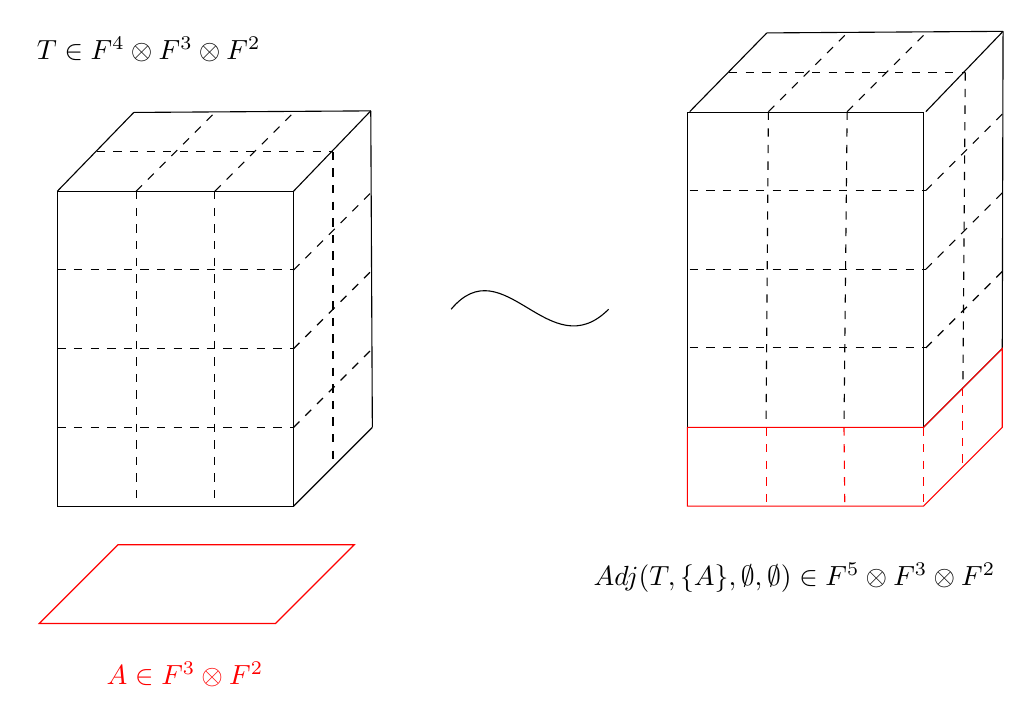
\begin{tikzpicture}[scale=1]
        % Coordinates
        \coordinate (A) at (1.00, 8.00);
        \coordinate (B) at (1.97, 9.00);
        \coordinate (C) at (4.00, 8.00);
        \coordinate (D) at (4.98, 9.02);
        \coordinate (E) at (4.00, 4.00);
        \coordinate (F) at (5.00, 5.00);
        \coordinate (G) at (1.50, 8.50);
        \coordinate (H) at (4.50, 8.50);
        \coordinate (I) at (4.50, 4.50);
        \coordinate (J) at (2.00, 8.00);
        \coordinate (K) at (2.00, 4.00);
        \coordinate (L) at (3.00, 8.00);
        \coordinate (M) at (3.00, 4.00);
        \coordinate (N) at (3.00, 9.00);
        \coordinate (O) at (4.00, 9.00);
        \coordinate (P) at (1.00, 7.00);
        \coordinate (Q) at (4.00, 7.00);
        \coordinate (R) at (5.00, 8.00);
        \coordinate (S) at (1.00, 6.00);
        \coordinate (T) at (4.00, 6.00);
        \coordinate (U) at (5.00, 7.00);
        \coordinate (V) at (1.00, 5.00);
        \coordinate (W) at (4.00, 5.00);
        \coordinate (X) at (5.00, 6.00);
        \coordinate (Y) at (2.16, 9.52);
        \coordinate (Z) at (9.03, 9.01);
        \coordinate (AA) at (10.01, 10.01);
        \coordinate (AB) at (12.03, 9.01);
        \coordinate (AC) at (13.01, 10.03);
        \coordinate (AD) at (12.00, 5.00);
        \coordinate (AE) at (13.00, 6.00);
        \coordinate (AF) at (9.53, 9.51);
        \coordinate (AG) at (12.53, 9.51);
        \coordinate (AH) at (12.50, 5.50);
        \coordinate (AI) at (10.03, 9.01);
        \coordinate (AJ) at (10.00, 5.00);
        \coordinate (AK) at (11.03, 9.01);
        \coordinate (AL) at (10.99, 5.00);
        \coordinate (AM) at (11.03, 10.01);
        \coordinate (AN) at (12.03, 10.01);
        \coordinate (AO) at (9.03, 8.01);
        \coordinate (AP) at (12.03, 8.01);
        \coordinate (AQ) at (13.03, 9.01);
        \coordinate (AR) at (9.03, 7.01);
        \coordinate (AS) at (12.03, 7.01);
        \coordinate (AT) at (13.03, 8.01);
        \coordinate (AU) at (9.03, 6.01);
        \coordinate (AV) at (12.03, 6.01);
        \coordinate (AW) at (13.03, 7.01);
        \coordinate (AX) at (0.77, 2.51);
        \coordinate (AY) at (3.77, 2.51);
        \coordinate (AZ) at (4.77, 3.51);
        \coordinate (BA) at (1.77, 3.51);
        \coordinate (BB) at (2.62, 1.58);
        \coordinate (BC) at (9.00, 5.00);
        \coordinate (BD) at (9.00, 4.00);
        \coordinate (BE) at (12.00, 4.00);
        \coordinate (BF) at (13.00, 5.00);
        \coordinate (BG) at (10.00, 4.00);
        \coordinate (BH) at (11.00, 4.00);
        \coordinate (BI) at (12.50, 4.50);
        \coordinate (BJ) at (10.36, 2.78);
        \coordinate (BK) at (6.00, 6.50);
        \coordinate (BL) at (8.00, 6.50);
        \coordinate (BM) at (6.67, 7.30);
        \coordinate (BN) at (7.25, 5.75);

        % Drawing
        \draw (1,4) rectangle (4,8);
        \draw (A) -- (B);
        \draw (C) -- (D);
        \draw (E) -- (F);
        \draw (B) -- (D);
        \draw (F) -- (D);
        \draw[dashed] (G) -- (H);
        \draw[dashed] (H) -- (I);
        \draw[dashed] (J) -- (K);
        \draw[dashed] (L) -- (M);
        \draw[dashed] (J) -- (N);
        \draw[dashed] (L) -- (O);
        \draw[dashed] (P) -- (Q);
        \draw[dashed] (Q) -- (R);
        \draw[dashed] (S) -- (T);
        \draw[dashed] (T) -- (U);
        \draw[dashed] (V) -- (W);
        \draw[dashed] (W) -- (X);
        \node[above] at (Y) {$T \in \mathbb{F}^4 \otimes \mathbb{F}^3 \otimes \mathbb{F}^2$};
        \draw (9,5) rectangle (12,9);
        \draw (Z) -- (AA);
        \draw (AB) -- (AC);
        \draw (AD) -- (AE);
        \draw (AA) -- (AC);
        \draw (AE) -- (AC);
        \draw[dashed] (AF) -- (AG);
        \draw[dashed] (AG) -- (AH);
        \draw[dashed] (AI) -- (AJ);
        \draw[dashed] (AK) -- (AL);
        \draw[dashed] (AI) -- (AM);
        \draw[dashed] (AK) -- (AN);
        \draw[dashed] (AO) -- (AP);
        \draw[dashed] (AP) -- (AQ);
        \draw[dashed] (AR) -- (AS);
        \draw[dashed] (AS) -- (AT);
        \draw[dashed] (AU) -- (AV);
        \draw[dashed] (AV) -- (AW);
        \draw[red] (AX) -- (AY) -- (AZ) -- (BA) -- cycle;
        \node[above, text=red] at (BB) {$A \in \mathbb{F}^3 \otimes \mathbb{F}^2
        $};
        \draw[red] (BC) -- (BD) -- (BE) -- (BF) -- (AE) -- (AD) -- cycle;
        \draw[red, dashed] (AJ) -- (BG);
        \draw[red, dashed] (AL) -- (BH);
        \draw[red, dashed] (AD) -- (BE);
        \draw[red, dashed] (AH) -- (BI);
        \node[above] at (BJ) {$Adj(T, \{A\}, \emptyset, \emptyset)\in \mathbb{F}^5\otimes\mathbb{F}^3\otimes\mathbb{F}^2$};
        \draw (BK) .. controls (6.67, 7.30) and (7.25, 5.75) .. (BL);
    \end{tikzpicture}
    \caption{Adjoining a slice $A$ to a tensor $T$}\label{figure:adjoiningslices}
\end{figure}
The \textbf{symmetric adjoin} can be denoted $SAdj(T, \mathcal{M})$ where $\mathcal{M}$ is adjoined along every mode, following the same process as given in \Cref{subsection:adjoiningprocedure}. 
% What does this operation look like in geometry?

The adjoining process as described creates a tensor of larger format, but the rank of such a tensor may be appropriately constrained depending on the slices being adjoined. It is this constraining property that Shitov \cite{shitov_higher_2024-1}  and Wang and Seigal \cite{wang_lower_2023} use to construct an intermediate tensor with adjoined slices that has a differing rank and symmetric rank.[IS THERE A PROOF? ILLUSTRATE/DEMONSTRATE]

\begin{remark}
    It may be trivial to note that while the order of the slices in $\mathcal{M}_i$ matters when constructing the final tensor, the rank information of the constructed tensor is independent of such changes in ordering. Further, the adjoining procedure itself can be modified, to follow any ordering of modes, as long as the slices required have been padded appropriately.
\end{remark}

\subsection{Generating Tensor Families modulo Slices}\label{subsection:familymoduloslices}
Given that a tensor can admit many non-unique decompositions, one way to analyse the structure of a tensor is via an analogy to Gaussian elimination for matrices. The substitution method as described in \cites{landsberg_abelian_2017,alexeev_tensor_2011} has been a computational tool for analysing tensors since the 1960's. Rather than arriving at one possible "lowest" optimal tensor, generating a family of tensors modulo a set of slices is equivalent to looking at all the possible ways a tensor could be transformed, based on transforming its constituent slices along different modes.

Defining such an operation that generates a linear span necessitates one additional, alternate description of padding a tensor into an appropriate format, now in terms of seeing the lower order slice as embedded into an empty higher order tensor. In doing so, it is also necessary to take a candidate higher order tensor as a "template" that the slice can be made to resemble. [REWRITE, CAN MAKE THIS DEFINITION SIMPLER. SIMPLY TENSOR WITH AN APPROPRIATE VECTOR ALONG THE MISSING MODE]
\begin{definition}[Padding an order-$(d-1)$ tensor into higher order]\label{defn:paddinghigherorder}
    Let $d > 0$, and $1 \leq i \leq d$. Let $T \in V_1 \otimes \cdots \otimes V_d$ be the candidate higher order tensor to be used as a template, and $A \in V_{\hat{i}}$ the order $d-1$ tensor to be padded into order $d$. 

    Then define $Pad_j^i: V_{\hat{i}} \times V \to V$ in coordinates as follows 
    $$Pad_j^i(A, T)(k_1, \ldots, k_d) = \begin{cases}
        A(k_1, \ldots, k_{i-1}, k_{i+1}, \ldots k_d) & k_i = j\\
        0 & \text{otherwise}
    \end{cases}$$
\end{definition}
\nomenclature[E]{$Pad^i_j(A, T)$}{The mapping taking a lower order tensor $A$ into the same format as a higher order tensor $T$, now seen as the only non-zero $j$-th slice along the $i$th mode (see \Cref{defn:paddinghigherorder})}
Equipped with this method of padding one can now define slicing a tensor $T$ along one particular mode.
\begin{definition}[Tensor Family Generated by Slices along a Mode]\label{defn:familymoduloslices}
    Let $d > 0$ and $1 \leq i \leq d$. Let $T \in V := V_1 \otimes \cdots \otimes V_d$ be an order-$d$ tensor, and $\mathcal{M} := \{M_1, \ldots, M_N\} \subset V_{\hat{i}}$ be a finite collection of order-$(d-1)$ slices of the appropriate format. 
    % Let $T \in V_1 \otimes \cdots \otimes V_d$ be an order $d$ tensor, and $A \in V_2 \otimes \cdots \otimes V_d$ such that $T = v_1 \otimes \cdots \otimes v_d$ and $A = a_2 \otimes \cdots \otimes a_d$.
    
    Define $Mod^i(T, \bar{\mathcal{M}}): V \times V_1 \otimes \cdots \otimes V_{i-1} \otimes \field^N \otimes V_{i+1} \otimes \cdots \otimes V_d \to 2^{V}$ in terms of coordinates as follows ($2^P$ denoting the power set of a set $P$):
    
    $$Mod^i(T, \bar{\mathcal{M}}) = \left\{T + \sum_{k=1}^{n_i}\sum_{j=1}^N\lambda_{j,k} Pad^i_k(S^i_j(\bar{\mathcal{M}})) \;|\; \lambda_{j,k} \in \field\right\}.$$
    Here slices are first selected from the constructed order-$d$ tensor from the family of lower-order tensors, then these are padded appropriately to remain of the same format as $T$, and then scaled and added to $T$.
    % Define $F:= T\mod(\{A\}, \emptyset, \ldots \emptyset)$ as the following family,
    % $$T + \sum_{j=1}^{n_1} \lambda_j e_j \otimes A, \;\lambda_j \in \mathbb{F}$$where each of the $e_j$ are the standard ordered basis vectors of $V_1$
\end{definition}
\nomenclature[E]{$Mod^i(T, \bar{\mathcal{M}})$}{The mapping generating a family of tensors by slicing $T$ with elements from $\mathcal{M}$ along the $i$th mode (see \Cref{defn:familymoduloslices})}
This definition can now be extended to performing this operation along all the $d$ modes. The only difference now notationally is writing $Mod^j(Mod^i(T, \bar{\mathcal{M}_i}), \bar{\mathcal{M}_j})$ to denote the $Mod^j(S, \bar{\mathcal{M}_j})$ for every $S \in Mod^i(T,\mathcal{M}_i)$ and then taking the union of all the resulting sets. Thus the final family $F := T\mod(\mathcal{M}_1, \ldots \mathcal{M}_d)$ is a result of the $d$-fold composition of the distinct $Mod^i$ operations.
\nomenclature[E]{$T\mod(\mathcal{M}_1, \ldots, \mathcal{M}_d)$}{The mapping denoting the family generated by slicing $T$ along each $i$-th mode with slices from $\mathcal{M}_i$}
\begin{proposition}\label{proposition:commutativemodulo} Let $T$ be an order-$d$ tensor $\in V_1 \otimes \cdots \otimes V_d$. Consider $\mathcal{M}_i \subset V_{\hat{i}}$and $\mathcal{M}_j \subset V_{\hat{j}}$ as collections of lower-order tensors of format appropriate to the $i$ and $j$ slices of $T$ respectively. Then the family generated modulo $\mathcal{M}_i$ and $\mathcal{M}_j$ is the same, regardless of which modulo operation is performed first, i.e.
    $$Mod^j(Mod^i(T, \bar{\mathcal{M}_i}), \bar{\mathcal{M}_j}) = Mod^i(Mod^j(T, \bar{\mathcal{M}_j}), \bar{\mathcal{M}_i})$$
\end{proposition}
\begin{proof}
   \begin{eqnarray*}
        &&Mod^j(Mod^i(T, \bar{\mathcal{M}_i}), \bar{\mathcal{M}_j}) \\
        &=& \left\{ Mod^j(S, \bar{\mathcal{M}_j}) | S \in Mod^i(T,\bar{\mathcal{M}_i}) \right\}\\
        &=& \left\{S + \sum_{a=1}^{n_j}\sum_{b=1}^{N_j}\lambda_{a,b} Pad^j_a(S^j_b(\bar{\mathcal{M}_j})) | \lambda_{a,b} \in \field, S \in Mod^i(T,\bar{\mathcal{M}_i}) \right\}\\
        &=& \left\{T + \sum_{c=1}^{n_i}\sum_{d=1}^{N_i}\lambda_{c,d} Pad^i_c(S^i_d(\bar{\mathcal{M}_i})) + \sum_{b=1}^{n_j}\sum_{a=1}^{N_j}\lambda_{a,b} Pad^j_a(S^j_b(\bar{\mathcal{M}_j})) | \lambda_{a,b}, \lambda_{c,d}\in \field \right\}\\
        &=& \left\{S + \sum_{c=1}^{n_i}\sum_{d=1}^{N_i}\lambda_{c,d} Pad^i_c(S^i_d(\bar{\mathcal{M}_i})) | \lambda_{c,d} \in \field, S \in Mod^j(T,\bar{\mathcal{M}_j}) \right\}\\
        &=& \left\{ Mod^i(S, \bar{\mathcal{M}_i}) | S \in Mod^j(T,\bar{\mathcal{M}_j}) \right\}\\
        &=& Mod^i(Mod^j(T, \bar{\mathcal{M}_j}), \bar{\mathcal{M}_i})
   \end{eqnarray*} 
\end{proof}
The above proof shows that the order of applying modulo operations on a given tensor does not affect the final resultant linear span.
\begin{observation}
    Here, the family $F \subseteq V_1 \otimes \cdots \otimes V_d$, i.e. all its elements remain of the same order as the original tensor $T$. \Cref{figure:familymoduloslices} illustrates how one one such element from such a family can be generated. [HOW/PROVIDE MORE DETAIL]
\end{observation}
\begin{remark}
    As with the adjoining operation for symmetric tensors, generating a family of symmetric tensors modulo symmetric slices also follows immediately from the definitions provided above, but in this case it is the same family of order-$(d-1)$ slices, $\mathcal{M}$,  being used along every mode. Therefore $T\mod\mathcal{M}:= T\mod(\mathcal{M}, \ldots, \mathcal{M}).$
\end{remark}
Since performing the modulo operation on a tensor gives a family instead of a single output tensor, one can talk about how the maximal or minimal rank of the tensor \textit{family} is affected.
% Geometrically what kind of linear span is this generating? In what space could such a span lie?
\begin{figure}
    \centering
    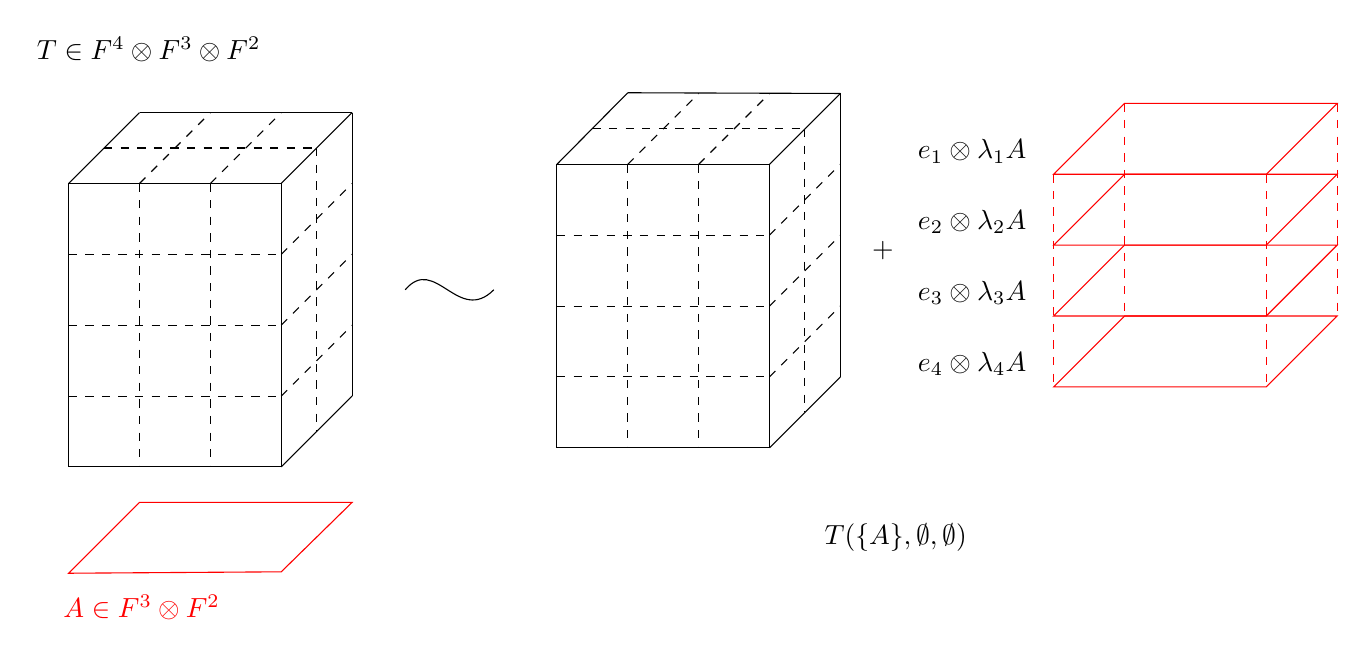
\begin{tikzpicture}[scale=0.9]
        % Coordinates
        \coordinate (A) at (1.00, 8.00);
        \coordinate (B) at (2.00, 9.00);
        \coordinate (C) at (4.00, 8.00);
        \coordinate (D) at (5.00, 9.00);
        \coordinate (E) at (4.00, 4.00);
        \coordinate (F) at (5.00, 5.00);
        \coordinate (G) at (1.50, 8.50);
        \coordinate (H) at (4.50, 8.50);
        \coordinate (I) at (4.50, 4.50);
        \coordinate (J) at (2.00, 8.00);
        \coordinate (K) at (2.00, 4.00);
        \coordinate (L) at (3.00, 8.00);
        \coordinate (M) at (3.00, 4.00);
        \coordinate (N) at (3.00, 9.00);
        \coordinate (O) at (4.00, 9.00);
        \coordinate (P) at (1.00, 7.00);
        \coordinate (Q) at (4.00, 7.00);
        \coordinate (R) at (5.00, 8.00);
        \coordinate (S) at (1.00, 6.00);
        \coordinate (T) at (4.00, 6.00);
        \coordinate (U) at (5.00, 7.00);
        \coordinate (V) at (1.00, 5.00);
        \coordinate (W) at (4.00, 5.00);
        \coordinate (X) at (5.00, 6.00);
        \coordinate (Y) at (2.13, 9.58);
        \coordinate (Z) at (1.00, 2.50);
        \coordinate (AA) at (4.00, 2.52);
        \coordinate (AB) at (5.00, 3.50);
        \coordinate (AC) at (2.00, 3.50);
        \coordinate (AD) at (2.03, 1.71);
        \coordinate (AE) at (7.89, 8.27);
        \coordinate (AF) at (8.89, 9.28);
        \coordinate (AG) at (10.89, 8.27);
        \coordinate (AH) at (11.89, 9.27);
        \coordinate (AI) at (10.89, 4.27);
        \coordinate (AJ) at (11.89, 5.27);
        \coordinate (AK) at (8.39, 8.77);
        \coordinate (AL) at (11.39, 8.77);
        \coordinate (AM) at (11.39, 4.77);
        \coordinate (AN) at (8.89, 8.27);
        \coordinate (AO) at (8.89, 4.27);
        \coordinate (AP) at (9.89, 8.27);
        \coordinate (AQ) at (9.89, 4.27);
        \coordinate (AR) at (9.89, 9.27);
        \coordinate (AS) at (10.89, 9.27);
        \coordinate (AT) at (7.89, 7.27);
        \coordinate (AU) at (10.89, 7.27);
        \coordinate (AV) at (11.89, 8.27);
        \coordinate (AW) at (7.89, 6.27);
        \coordinate (AX) at (10.89, 6.27);
        \coordinate (AY) at (11.89, 7.27);
        \coordinate (AZ) at (7.89, 5.27);
        \coordinate (BA) at (10.89, 5.27);
        \coordinate (BB) at (11.89, 6.27);
        \coordinate (BC) at (14.90, 8.13);
        \coordinate (BD) at (17.90, 8.13);
        \coordinate (BE) at (18.90, 9.13);
        \coordinate (BF) at (15.90, 9.13);
        \coordinate (BG) at (14.90, 7.13);
        \coordinate (BH) at (17.90, 7.13);
        \coordinate (BI) at (18.90, 8.13);
        \coordinate (BJ) at (15.90, 8.13);
        \coordinate (BK) at (14.90, 6.13);
        \coordinate (BL) at (17.90, 6.13);
        \coordinate (BM) at (18.90, 7.13);
        \coordinate (BN) at (15.90, 7.13);
        \coordinate (BO) at (14.90, 5.13);
        \coordinate (BP) at (17.90, 5.13);
        \coordinate (BQ) at (18.90, 6.13);
        \coordinate (BR) at (15.90, 6.13);
        \coordinate (BS) at (5.75, 6.50);
        \coordinate (BT) at (7.00, 6.50);
        \coordinate (BU) at (6.17, 7.00);
        \coordinate (BV) at (6.50, 6.00);
        \coordinate (BW) at (12.49, 6.78);
        \coordinate (BX) at (13.75, 8.15);
        \coordinate (BY) at (13.75, 7.15);
        \coordinate (BZ) at (13.75, 6.15);
        \coordinate (CA) at (13.75, 5.15);
        \coordinate (CB) at (12.67, 2.67);

        % Drawing
        \draw (1,4) rectangle (4,8);
        \draw (A) -- (B);
        \draw (C) -- (D);
        \draw (E) -- (F);
        \draw (B) -- (D);
        \draw (F) -- (D);
        \draw[dashed] (G) -- (H);
        \draw[dashed] (H) -- (I);
        \draw[dashed] (J) -- (K);
        \draw[dashed] (L) -- (M);
        \draw[dashed] (J) -- (N);
        \draw[dashed] (L) -- (O);
        \draw[dashed] (P) -- (Q);
        \draw[dashed] (Q) -- (R);
        \draw[dashed] (S) -- (T);
        \draw[dashed] (T) -- (U);
        \draw[dashed] (V) -- (W);
        \draw[dashed] (W) -- (X);
        \node[above] at (Y) {$T \in \mathbb{F}^4 \otimes \mathbb{F}^3 \otimes \mathbb{F}^2$};
        \draw[red] (Z) -- (AA) -- (AB) -- (AC) -- cycle;
        \node[above, text=red] at (AD) {$A \in \mathbb{F}^3 \otimes \mathbb{F}^2$};
        \draw (7.89,4.27) rectangle (10.89,8.27);
        \draw (AE) -- (AF);
        \draw (AG) -- (AH);
        \draw (AI) -- (AJ);
        \draw (AF) -- (AH);
        \draw (AJ) -- (AH);
        \draw[dashed] (AK) -- (AL);
        \draw[dashed] (AL) -- (AM);
        \draw[dashed] (AN) -- (AO);
        \draw[dashed] (AP) -- (AQ);
        \draw[dashed] (AN) -- (AR);
        \draw[dashed] (AP) -- (AS);
        \draw[dashed] (AT) -- (AU);
        \draw[dashed] (AU) -- (AV);
        \draw[dashed] (AW) -- (AX);
        \draw[dashed] (AX) -- (AY);
        \draw[dashed] (AZ) -- (BA);
        \draw[dashed] (BA) -- (BB);
        \draw[red] (BC) -- (BD) -- (BE) -- (BF) -- cycle;
        \draw[red] (BG) -- (BH) -- (BI) -- (BJ) -- cycle;
        \draw[red] (BK) -- (BL) -- (BM) -- (BN) -- cycle;
        \draw[red] (BO) -- (BP) -- (BQ) -- (BR) -- cycle;
        \draw (BS) .. controls (6.17, 7.00) and (6.50, 6.00) .. (BT);
        \draw[red, dashed] (BC) -- (BO);
        \draw[red, dashed] (BF) -- (BR);
        \draw[red, dashed] (BD) -- (BP);
        \draw[red, dashed] (BE) -- (BQ);
        \node[above] at (BW) {$+$};
        \node[above] at (BX) {$e_1 \otimes \lambda_1A$};
        \node[above] at (BY) {$e_2 \otimes \lambda_2A$};
        \node[above] at (BZ) {$e_3 \otimes \lambda_3A$};
        \node[above] at (CA) {$e_4 \otimes \lambda_4A$};
        \node[above] at (CB) {$T\mod(\{A\}, \emptyset, \emptyset)$};
        \end{tikzpicture}
    \caption{Family generated from a tensor $T$ by a slice $A$}\label{figure:familymoduloslices}
\end{figure}
\subsection*{Combining Adjoining and Modulo}
% What does introducing such a combination of operations allow us to do? What does this tell us about either construction?
As seen in the previous two subsections, rank information of a tensor does change when adjoining slices, and the following theorem is becomes important in Wang and Seigal's 2023 paper \cite{seigal_ranks_2020}.
\begin{theorem}[\cite{wang_lower_2023}]\label{thm:computingrankpostadjoin}
    Suppose $T \in V:= V_1 \otimes \cdots \otimes V_d$ is an order-$d$ tensor, and $\mathcal{M}_i \subset V_{\hat{i}}$ for every $1 \leq i \leq d$. Then $$\rank( Adj(T, \mathcal{M}_1, \ldots, \mathcal{M}_d)) \geq \min \rank (T\mod(\mathcal{M}_1, \ldots, \mathcal{M}_d)) + \sum_{j=1}^{d} \dim \langle \mathcal{M}_j\rangle$$
    Equality holds if each of the $\mathcal{M}_i$ consist of only rank-one tensors.
\end{theorem}
[ADD PROOF]
\subsection{Cloning Tensors}\label{subsection:tensorcloning}
The idea of cloning a tensor is born out of necessity. When constructing an emulating family (see \Cref{subsection:emulatingfamily}), difficulties arise when working with tensors of a fixed, finite format. Cloning a tensor, as the name suggests, seeks to preserve the properties of the original, while embedding it in a much "larger space".
\begin{definition}[Cloning a Tensor]\label{defn:tensorcloning}
    Fix $d > 0$. Let $T \in V:= V_1 \otimes \cdots \otimes V_d$ be an order-$d$ tensor.
    
    The $n$-th cloning function $C_n: V \to \left(\bigoplus_{i=1}^n V_1\right) \otimes \cdots \otimes \left(\bigoplus_{i=1}^n V_d\right)$ can be defined in coordinates in the following manner: $$C_n(T)(k_{1, j_1}, \ldots, k_{d, j_d}) = T(k_1, \ldots, k_d).$$Here, the notation $k_{i,j_i}:= k_{(j_i-1)n + i}$. where $1 \leq j_i \leq n$.
    % Define the $n$ clone of $T:= C_n(T)$ as $$C_n(T)(k_{1, j_1}, \ldots, k_{d, j_d}) = T(k_1, \ldots, k_d),$$where $1 \leq j_i \leq n$. The notation $k_{i,j}$ denotes $k_{(j-1)n + i}$.
\end{definition}
\nomenclature[E]{$C_n(T)$}{The mapping that constructs the $n$-th clone of a tensor $T$}
\begin{observation}
    % It can be seen that $C_n(T) \in \left(\bigoplus_{i=1}^n V_1\right) \otimes \cdots \otimes \left(\bigoplus_{i=1}^n V_d\right)$, an indication that cloning is merely a repeated copying operation.
    Since the definition of cloning depends on a non-zero $d$, one can clone tensors of any order, in particular vectors, as well. This leads to the description of the clone of a standard ordered basis vector $e_i \in V$, an $\field$ vector space as: $C_n(e_i) = \sum_{j=1}^{n} e_{i,j}.$
\end{observation} 
\begin{figure}
    \centering
    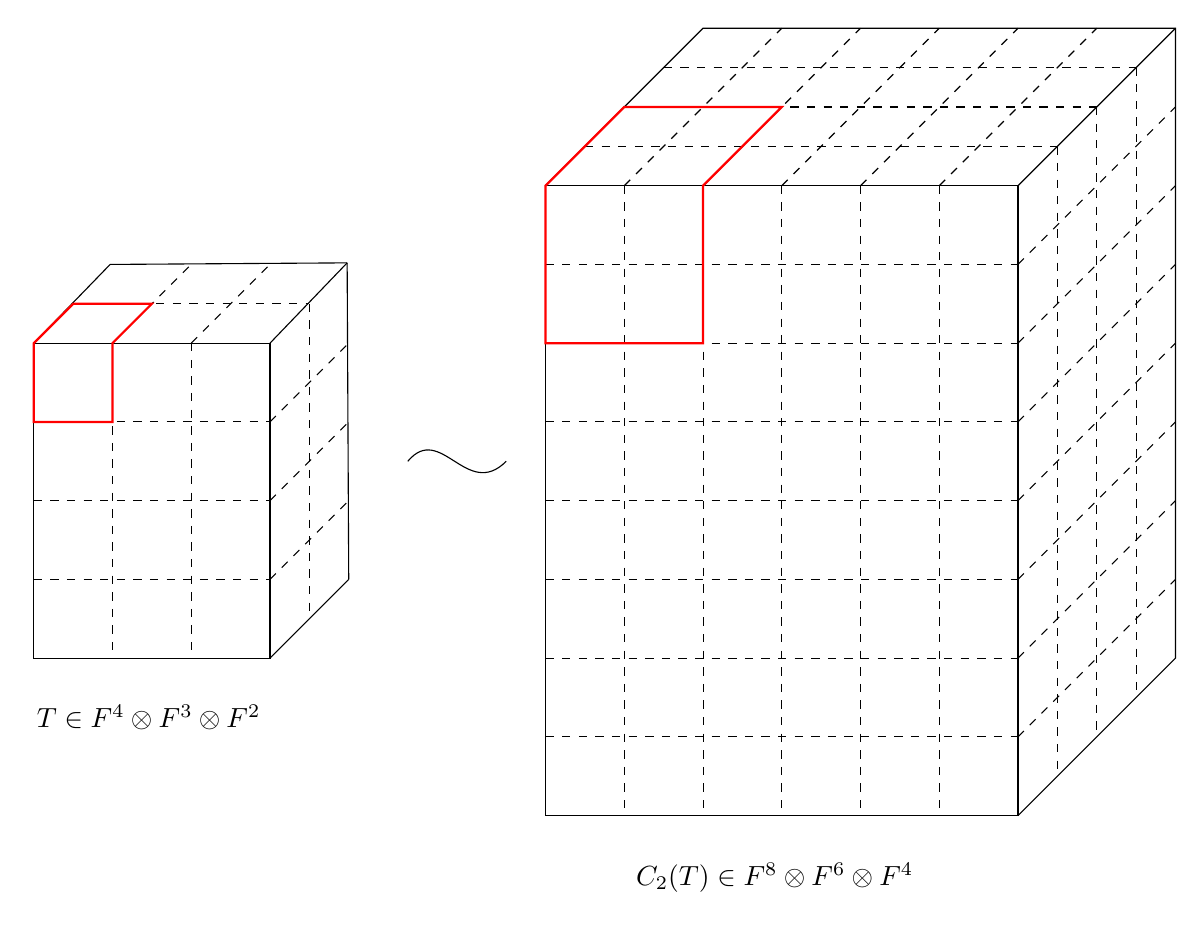
\begin{tikzpicture}[scale=1]
        % Coordinates
        \coordinate (A) at (1.00, 8.00);
        \coordinate (B) at (1.97, 9.00);
        \coordinate (C) at (4.00, 8.00);
        \coordinate (D) at (4.98, 9.02);
        \coordinate (E) at (4.00, 4.00);
        \coordinate (F) at (5.00, 5.00);
        \coordinate (G) at (1.50, 8.50);
        \coordinate (H) at (4.50, 8.50);
        \coordinate (I) at (4.50, 4.50);
        \coordinate (J) at (2.00, 8.00);
        \coordinate (K) at (2.00, 4.00);
        \coordinate (L) at (3.00, 8.00);
        \coordinate (M) at (3.00, 4.00);
        \coordinate (N) at (3.00, 9.00);
        \coordinate (O) at (4.00, 9.00);
        \coordinate (P) at (1.00, 7.00);
        \coordinate (Q) at (4.00, 7.00);
        \coordinate (R) at (5.00, 8.00);
        \coordinate (S) at (1.00, 6.00);
        \coordinate (T) at (4.00, 6.00);
        \coordinate (U) at (5.00, 7.00);
        \coordinate (V) at (1.00, 5.00);
        \coordinate (W) at (4.00, 5.00);
        \coordinate (X) at (5.00, 6.00);
        \coordinate (Y) at (7.50, 10.00);
        \coordinate (Z) at (9.50, 12.00);
        \coordinate (AA) at (15.50, 12.00);
        \coordinate (AB) at (15.50, 4.00);
        \coordinate (AC) at (13.50, 2.00);
        \coordinate (AD) at (13.50, 10.00);
        \coordinate (AE) at (8.50, 10.00);
        \coordinate (AF) at (10.50, 12.00);
        \coordinate (AG) at (9.50, 10.00);
        \coordinate (AH) at (11.50, 12.00);
        \coordinate (AI) at (10.50, 10.00);
        \coordinate (AJ) at (12.50, 12.00);
        \coordinate (AK) at (11.50, 10.00);
        \coordinate (AL) at (13.50, 12.00);
        \coordinate (AM) at (12.50, 10.00);
        \coordinate (AN) at (14.50, 12.00);
        \coordinate (AO) at (8.50, 2.00);
        \coordinate (AP) at (9.50, 2.00);
        \coordinate (AQ) at (10.50, 2.00);
        \coordinate (AR) at (11.50, 2.00);
        \coordinate (AS) at (12.50, 2.00);
        \coordinate (AT) at (8.00, 10.50);
        \coordinate (AU) at (14.00, 10.50);
        \coordinate (AV) at (8.50, 11.00);
        \coordinate (AW) at (14.50, 11.00);
        \coordinate (AX) at (9.00, 11.50);
        \coordinate (AY) at (15.00, 11.50);
        \coordinate (AZ) at (7.50, 9.00);
        \coordinate (BA) at (13.50, 9.00);
        \coordinate (BB) at (7.50, 8.00);
        \coordinate (BC) at (13.50, 8.00);
        \coordinate (BD) at (7.50, 7.00);
        \coordinate (BE) at (13.50, 7.00);
        \coordinate (BF) at (7.50, 6.00);
        \coordinate (BG) at (13.50, 6.00);
        \coordinate (BH) at (7.50, 5.00);
        \coordinate (BI) at (13.50, 5.00);
        \coordinate (BJ) at (7.50, 4.00);
        \coordinate (BK) at (13.50, 4.00);
        \coordinate (BL) at (7.50, 3.00);
        \coordinate (BM) at (13.50, 3.00);
        \coordinate (BN) at (15.50, 11.00);
        \coordinate (BO) at (15.50, 10.00);
        \coordinate (BP) at (15.50, 9.00);
        \coordinate (BQ) at (15.50, 8.00);
        \coordinate (BR) at (15.50, 7.00);
        \coordinate (BS) at (15.50, 6.00);
        \coordinate (BT) at (15.50, 5.00);
        \coordinate (BU) at (14.00, 2.50);
        \coordinate (BV) at (14.50, 3.00);
        \coordinate (BW) at (15.00, 3.50);
        \coordinate (BX) at (2.00, 7.00);
        \coordinate (BY) at (2.50, 8.50);
        \coordinate (BZ) at (9.50, 8.00);
        \coordinate (CA) at (10.50, 11.00);
        \coordinate (CB) at (5.75, 6.50);
        \coordinate (CC) at (7.00, 6.50);
        \coordinate (CD) at (6.17, 7.00);
        \coordinate (CE) at (6.50, 6.00);
        \coordinate (CF) at (2.46, 2.97);
        \coordinate (CG) at (10.41, 0.90);

        % Drawing
        \draw (1,4) rectangle (4,8);
        \draw (A) -- (B);
        \draw (C) -- (D);
        \draw (E) -- (F);
        \draw (B) -- (D);
        \draw (F) -- (D);
        \draw[dashed] (G) -- (H);
        \draw[dashed] (H) -- (I);
        \draw[dashed] (J) -- (K);
        \draw[dashed] (L) -- (M);
        \draw[dashed] (J) -- (N);
        \draw[dashed] (L) -- (O);
        \draw[dashed] (P) -- (Q);
        \draw[dashed] (Q) -- (R);
        \draw[dashed] (S) -- (T);
        \draw[dashed] (T) -- (U);
        \draw[dashed] (V) -- (W);
        \draw[dashed] (W) -- (X);
        \draw (7.5,2) rectangle (13.5,10);
        \draw (Y) -- (Z) -- (AA) -- (AB) -- (AC);
        \draw (AD) -- (AA);
        \draw[dashed] (AE) -- (AF);
        \draw[dashed] (AG) -- (AH);
        \draw[dashed] (AI) -- (AJ);
        \draw[dashed] (AK) -- (AL);
        \draw[dashed] (AM) -- (AN);
        \draw[dashed] (AE) -- (AO);
        \draw[dashed] (AG) -- (AP);
        \draw[dashed] (AI) -- (AQ);
        \draw[dashed] (AK) -- (AR);
        \draw[dashed] (AM) -- (AS);
        \draw[dashed] (AT) -- (AU);
        \draw[dashed] (AV) -- (AW);
        \draw[dashed] (AX) -- (AY);
        \draw[dashed] (AZ) -- (BA);
        \draw[dashed] (BB) -- (BC);
        \draw[dashed] (BD) -- (BE);
        \draw[dashed] (BF) -- (BG);
        \draw[dashed] (BH) -- (BI);
        \draw[dashed] (BJ) -- (BK);
        \draw[dashed] (BL) -- (BM);
        \draw[dashed] (BA) -- (BN);
        \draw[dashed] (BC) -- (BO);
        \draw[dashed] (BE) -- (BP);
        \draw[dashed] (BG) -- (BQ);
        \draw[dashed] (BI) -- (BR);
        \draw[dashed] (BK) -- (BS);
        \draw[dashed] (BM) -- (BT);
        \draw[dashed] (AU) -- (BU);
        \draw[dashed] (AW) -- (BV);
        \draw[dashed] (AY) -- (BW);
        \draw[red, thick] (P) -- (BX) -- (J) -- (BY) -- (G) -- (A) -- cycle;
        \draw[red, thick] (Y) -- (BB) -- (BZ) -- (AG) -- (CA) -- (AV) -- cycle;
        \draw (CB) .. controls (6.17, 7.00) and (6.50, 6.00) .. (CC);
        \node[above] at (CF) {$T \in \mathbb{F}^4\otimes\mathbb{F}^3\otimes\mathbb{F}^2$};
        \node[above] at (CG) {$C_2(T) \in \mathbb{F}^8\otimes\mathbb{F}^6\otimes\mathbb{F}^4
        $};
    \end{tikzpicture}
    \caption{$2$ clone of a tensor $T$}\label{figure:cloningtensor}
\end{figure}

\begin{lemma}\label{lemma:cloningdistribution}
    The cloning operation as defined above distributes over the tensor product i.e. $C_n(A \otimes B) = C_n(A) \otimes C_n(B)$ where $A, B$ are vectors in an arbitrary vector space.
\end{lemma}
\begin{proof}
    Consider two arbitrary vectors, $A := (a_1, \ldots, a_k), B := (b_1, \ldots, b_k) \in V$, an $\field$ vector space. Then $A \otimes B$ is an order $2$ tensor (a matrix) lying in $V \otimes V$, and $(A \otimes B)(i,j) = a_ib_j$
    Then according to \Cref{defn:tensorcloning}, $$C_n(A \otimes B)(k_1,k_2) = (A \otimes B)(k_1(\mod n), k_2(\mod n)) = A(k_1(\mod n))B(k_2(\mod n)),$$ here using the regular modulo operation from number theory. This tensor lies in $\left(\bigoplus_{i=1}^n V\right) \otimes \left(\bigoplus_{i=1}^n V\right)$.

    Now taking the vectors $C_n(A), C_n(B) \in \left(\bigoplus_{i=1}^n V\right)$. Here $$C_n(A) = (\underbrace{a_1, \ldots, a_1}_{\text{$n$ times}}, \ldots \underbrace{a_k, \ldots, a_k}_{\text{$n$ times}}),$$ and likewise for $C_n(B)$. Their tensor product is also a matrix lying in $\left(\bigoplus_{i=1}^n V\right) \otimes \left(\bigoplus_{i=1}^n V\right)$ where now $$(C_n(A) \otimes C_n(B))(k_1, k_2) = C_n(A)(k_1)C_n(B)(k_2) = A(k_1(\mod n))B(k_2(\mod n)).$$Thus, since each component of both tensors is equal, they are the same tensor.
\end{proof}
\begin{remark}
    For two tensors $A, B$ to show that cloning distributes over the tensor product $A \otimes B$ is a little more involved. However this problem simplifies to asking whether $C_n(a \otimes b \otimes c) = C_n(a) \otimes C_n(b) \otimes C_n(c)$ where $a, b, c$ are vectors. This simplified problem can be solved in the same way as the proof above, by working in coordinates and using the modulo function from number theory.
\end{remark}
Another description of cloning is by first transforming the tensor under consideration in the following manner. Denote $\mathbf{1}_n$ as the vector of 1's lying in $\field^n$. Then the $n$-clone of a simple vector $v$ can be described as $(v \otimes \mathbf{1}_n)^{\emptyset}$ or the flattening of the matrix created by tensoring $v$ with the vector of ones. Thus another way to look at $C_n(T)$ is with the following procedure: 

\begin{eqnarray*}
    C_n(T) &=& C_n\left(\sum_{i=1}^{r} T_i\right)\\
    &=& \sum_{i=1}^{r} C_n(T_i)\\
    &=& \sum_{i=1}^{r} C_n(v^i_1 \otimes \cdots \otimes v^i_d)\\
    &=& \sum_{i=1}^{r} C_n(v^i_i) \otimes \cdots \otimes C_n(v^i_d)\\
    &=& \sum_{i=1}^{r} (v^i_1 \otimes \mathbf{1}_n)^{\emptyset} \otimes \cdots \otimes (v^i_d \otimes \mathbf{1}_n)^{\emptyset}
\end{eqnarray*}
\begin{remark}
    This property, along with the observation that cloning is a linear operation, allows for the proof that cloning a tensor does preserve its rank.
\end{remark} 
\nomenclature[C]{$\mathbf{1}_n$}{The vector of all $1$'s lying in $\field^n$}
\begin{proposition}
    $\rank(T) = \rank(C_n(T))$ for $C_n$ the cloning operation as defined in \Cref{defn:tensorcloning}, and $T \in V:= V_1 \otimes \cdots \otimes V_d$.
\end{proposition} 
\begin{proof}The proof is straightforward, and is as follows
    \begin{description}
        \item[$\leq$:] Since $T$ can be seen as a sub-tensor lying in $C_n(T)$, this inequality naturally exists. The rank of a subtensor is always at most the rank of the tensor, but never more.
        \item[$\geq$:] Since cloning distributes over addition (\Cref{lemma:cloningdistribution}), if  one has the rank decomposition $T = \sum_{i=1}^{r} T_i$, then $C_n(T) = \sum_{i=1}^{r} C_n(T_i)$ is a decomposition of $C_n(T)$. Thus the rank of $C_n(T)$ is at most that of $T$.  
    \end{description}
\end{proof}
\section{The Counterexample over $\reals$}\label{section:seigalcounterexample}
Wang and Seigal \cite{wang_lower_2023} in 2023 published a paper that demonstrated the construction of a distinct counterexample to Comon's conjecture, following Shitov \cite{shitov_comons_2020}. Their paper first examined the constructions made by Shitov, established new notation and terminology to prove results on rank pre- and post-operations, and finally they used MATLAB to construct a distinct order-$6$ example with real rank $30913$ and real symmetric rank $30914$. 

As the title of the paper suggests, such a counterexample relies on certain lower bounds and inequalities remaining strict, particularly when making constructions in a field (namely $\reals$) that is not algebraically complete. 
\subsection{Details from the Paper}\label{subsection:seigaldetails}
The paper in 2023 \cite{wang_lower_2023} works over $\reals$, specifically in $\reals[x,y]$ as the underlying ring of polynomials from which the homogenous polynomials can be selected. For simplicity's sake, there are only 2 variables, corresponding to an underlying real vector space of dimension $2$. 

The particular tensor under consideration is represented by the homogenous polynomial $x^d - ky^d$ where $d > 0$ is a fixed, even integer, and $k > 0$ (also fixed). Such a homogenous polynomial corresponds to the following tensor \begin{equation}\label{eqn:wangoriginaltensor}
    T:= (e_1)^{\otimes d} - k (e_2)^{\otimes d}, k > 0 , d = 2n, n \in \integer_+
\end{equation}
Visualised as a multiway array, this is a tensor that has non-zero entries at the two extreme "corners" and 0's everywhere else. Such a tensor clearly has rank and symmetric rank as $2$. 

Since the stated goal is to construct a counterexample to Comon's conjecture, this initial "seed" tensor, $T$, is first modified by the using a specific family of slices to generate a linear span of tensors (see \Cref{subsection:familymoduloslices}). Such a family when constructed has elements having minimal rank and symmetric rank. The elements in this family achieiving these minimal values do not have to be the same.

The family chosen in this case is \begin{equation}\label{eqn:wangslicingfamilypoly}
    \mathcal{M} := \{ x^{d-1-i}y^i \}_{i = 1}^{d-2}
\end{equation}This is a collection of monomials of degree $(d-1)$ that are of \textit{mixed} form i.e. they are monomials not purely in either variable. When describing such a family in terms of symmetric tensors (see \Cref{subsection:homogenouspolyrelation}), the family can be written as \begin{equation}\label{eqn:wangslicingfamilytensor}
    \mathcal{M} := \left\{ \frac{1}{(d-1)!} \sum_{\sigma \in S_{d-1}} \sigma((e_1)^{\otimes d-1-i}\otimes (e_2)^{\otimes i})\right\}_{i = 1}^{d-2}
\end{equation}
These order-$(d-1)$ tensors, since they are not formed of a single standard ordered basis vector, they do not affect the initial tensor $T$, when performing the operation of generating a family modulo slices: $T\mod\mathcal{M}$. (Note here since they are working with symmetric tensors, it is enough to specify only one family.)

\subsection*{Establishing A Difference in Rank and Symmetric Rank}
Within the constructed family $T\mod\mathcal{M}$, a tensor $P \in T\mod\mathcal{M}$ corresponds to the following polynomial \begin{equation}\label{eqn:orderdelementinconstructedfamily}
    P(x,y) := x^d - ky^d + \sum_{i=1}^{d-2} (\alpha_i x + \beta_i y)x^{d-1-i}y^i,
    \alpha_i, \beta_i \in \reals \forall i = 1,\ldots,d-2, k > 0 
\end{equation} 
First, the symmetric rank decomposition is computed, and shown to be at least 2 or higher. 
\begin{proposition}[\cite{wang_lower_2023}]
    A polynomial of the form $P(x,y)$ (as \Cref{eqn:orderdelementinconstructedfamily}) has symmetric rank at least 2. 
\end{proposition}
\begin{proof}
    Suppose not. Then one can rewrite $P(x,y)$ in terms of a linear polynomial raised to the $d$th power i.e.
    $$P(x,y) = (ax + by)^d$$for some choices of $a,b \in \reals$.\\ Expanding the RHS would then lead to the following 
    \begin{eqnarray*}
        P(x,y) &=& (ax + by)^d\\
        &=& \sum_{j=0}^{d}\binom{d}{j} a^{d-j}b^jx^{d-j}y^j.\\ 
    \end{eqnarray*}This leads to the following equality of polynomial expressions:
    
    $$x^d - ky^d + \sum_{i=1}^{d-2} (\alpha_i x + \beta_i y)x^{d-1-i}y^i = \sum_{j=0}^{d}\binom{d}{j} a^{d-j}b^jx^{d-j}y^j.$$
    
    This leads to a contradiction simply by looking at the coefficient of the $y^d$ monomial on either side of the equality. One must have $b^d = -k$ for some choice of $b \in \reals$.
    Since such an equation has no real solutions, the initial assumption of being able to write $P$ in terms of the $d$-th power of a single linear form was false, and therefore the Waring rank (equivalent to the symmetric rank) of $P \geq 2$.
\end{proof}
This establishes $\min_{P \in T\mod\mathcal{M}} \srank(P) = 2$. The next step in the paper is the establishing of the fact that the minimum \textit{rank} element of such a family has rank $1$.
\begin{proposition}[\cite{wang_lower_2023}]
    There is a tensor of the form $P(x,y)$ (see \Cref{eqn:orderdelementinconstructedfamily}) that is an elementary tensor 
\end{proposition}
\begin{proof}
    Consider the original tensor $T := x^d - ky^d$ (see \Cref{eqn:wangoriginaltensor}). This is a tensor of the form as in \Cref{eqn:orderdelementinconstructedfamily}. Now summing all the elements in $\mathcal{M}$ as defined earlier (see \Cref{eqn:wangslicingfamilypoly}) gives an order $d-1$ tensor with non-zero entries everywhere except for two "corners" --- corresponding to $x^{d-1}$ and $y^{d-1}$. These can be added along the $d$-th mode to the first slice, and after scaling by a factor of $-k$, to the last slice.
   
    Formally the tensor $T$ is now modified to $$x^d - ky^d + \underbrace{\sum_{i=1}^{d-2} x^{d-i}y^i}_{\text{modifying the first $d$-slice}} + \underbrace{-k\left(\sum_{j=1}^{d-2} x^{d-1-j}y^{j+1}\right)}_{\text{scaling and modifying the last $d$-slice}}$$An important point to note here is that changing the degree of the polynomial changes the order, and since the tensors all lie in $(\reals^2)^{\otimes d}$, changes affecting the "first" slice have an extra factor of $x$, and changes affecting the "last" or second have an extra factor of $y$.

    The final step of construction is adding the order-$(d-1)$ tensor corresponding to the monomial $x^{d-2}y$ (scaled by an appropriate $a_i$) to the first $i$-slice for all $d$ modes of the tensor $T$. Likewise for the tensor corresponding to the monomial $xy^{d-2}$ (with appropriate $b_i$ added to the last $i$-slices). The choices of these scaling coefficients are such that the following conditions are satisfied: \begin{eqnarray}
        \left(\sum_{i=1}^{d} a_i\right) - a_j &=& 0, \forall j \neq d\\
        \sum_{i=1}^{d-1} a_i  &=& -k\\
        \left(\sum_{i=1}^{d} b_i\right) - b_j &=& 0, \forall j \neq d\\
        \sum_{i=1}^{d-1} b_i  &=& 1
    \end{eqnarray}
    These choices for $a_i$ are made because modifying the tensor by adding the scaled tensors modifies only one entry in last $d$ slice. The last addition of $x^{d-1}y$ along the $d$-mode only affects the first $d$-slice. A similar line of reasoning follows the choices for the $b_i$. Making such choices is always possible, and non-unique.

    Performing these operations results in a tensor still lying in the family $T\mod \mathcal{M}$, now of the form $(\mathbf{1}_2)^{\otimes d-1} \otimes (1, -k)$, an elementary order $d$ tensor. Here again $\mathbf{1}_n$ denotes the vector of all $1$'s lying in $\field^n$
\end{proof}
\begin{remark}
    It is useful to note that proving such an elementary tensor exists is not a function of the underlying field. (assuming characteristic 0). Such a proof could also be modified for any number of variables (moving from working in $\field^2$ to $\field^n$), and for tensors of any even order $d$.
\end{remark}
The following statement holds for the family $T\mod\mathcal{M}$ \begin{equation}\label{eqn:familyineq}
    \min \rank (T\mod\mathcal{M}) < \min \srank (T\mod\mathcal{M})
\end{equation}

\subsection*{Moving from Families to a Specific Tensor}
Now that the existence of a family having elements with differing minimal rank and symmetric rank has been established, the authors construct $SAdj(T, \mathcal{M})$, as a symmetric tensor that is a candidate counterexample to Comon's conjecture. The problem of computing the rank of such a construction now arises, as it relates to the original $T$ and candidate family $\mathcal{M}$. 

The solution proposed originally by Shitov \cite{shitov_comons_2020}, is a proposed modification of $\mathcal{M}$ to a family of \textit{elementary} order $(d-1)$ tensors that span the same linear space [WHY? SPECIFIED EARLIER?]. Unfortunately, in the format $(\reals^2)^{\otimes 4}$, doing so also violates the vital inequality required for rank and symmetric rank of the family $T \mod \mathcal{M}$ (see \Cref{eqn:familyineq}).

Such a modification is required for the original computation of rank (see \Cref{thm:computingrankpostadjoin}) to be an equality (because equality only holds when the family consists of elementary tensors). 

[REWORK THIS WHOLE SECTION + PROOF]
The following proposition as adapted from \cite{wang_lower_2023}, shows that for higher order examples (viz. order $2n$ where $n > 2$), simply modifying Shitov's argument from the order $4$ case does not work i.e. it may be possible to modify the family $\mathcal{M}$ to elementary tensors that preserves the inequality in \Cref{eqn:familyineq}.  
\begin{proposition}\label{prop:modifyingfamily}
    Consider $T$ as in \Cref{eqn:wangoriginaltensor}, and $\mathcal{M}$ as \Cref{eqn:wangslicingfamilypoly}. Let $\mathcal{W} \subset (\reals^2)^{\otimes d-1}$, a finite set of elementary symmetric tensors such that $\mathcal{W}$ spans $\mathcal{M}$. Then the argument that $0 \in T \mod \mathcal{W}$ when $d = 2n, n > 2$ from \cite{wang_lower_2023} does not hold.
\end{proposition}
\begin{proof}
    Consider $\mathcal{W}$, a collection of elementary symmetric tensors of appropriate order. Showing $0 \in T\mod\mathcal{W}$ is equivalent to asking that $\mathcal{W}$ spans the set $\{x^iy^{d-i}\}_{i=0}^{d-1} \supseteq \mathcal{M}$ This is due to the fact that every slice of $T$ (seen as an order-$(d-1)$ tensor and therefore represented by a degree-$(d-1)$ polynomial) can then be expressed as lying in the span of $\mathcal{W}$. In particular, if one can show that the dimension of span $\mathcal{W}$ is $d$ (the number of degree $d-1$ monomials in 2 variables), this completes the proof that would show that the inequality in \Cref{eqn:familyineq} is violated.

    Suppose the dimension of the span of $\mathcal{W}$ is less than $d$. 
    Consider the tensor represented by $x^{d-2}y$. This monomial has rank $d-1$ since it can be written minimally as sum of $d-1$ elementary tensors. Thus the dimension of span $\mathcal{W}$ is at least $d-1$. Since $\mathcal{W}$ consists of symmetric tensors, its basis vectors must be a linear forms raised to the $d-1$th power: $(\lambda_ix + \mu_iy)^{d-1}$. These forms must also correspond to elementary tensors, by virtue of being elements of $\mathcal{W}$. 

    Now since this set, $\{ (\lambda_ix + \mu_iy)^{d-1}\}_{i=1}^{d-1}$ is a basis for span $\mathcal{W} \supseteq \mathcal{M}$, one must have that the tensors $x^{d-2}y$ and $xy^{d-2}$ can be written as linear combinations of the elements of the set. Doing so imposes conditions on $\lambda_i, \mu_i > 0$ such that $$\sum_{i=1}^d \frac{\lambda_i}{\mu_i} = 0 = \sum_{i=1}^d \frac{\mu_i}{\lambda_i}.$$
    This set of equalities results in the statement $$1 = \frac{\lambda_1}{\mu_1}\frac{\mu_1}{\lambda_1} = \left(\sum_{i=2}^d \frac{\lambda_i}{\mu_i}\right)\left(\sum_{i=2}^d \frac{\mu_i}{\lambda_i}\right) = (d-1) + \sum_{i=2}^d \sum_{j\neq i} \frac{\lambda_i\mu_j}{\mu_i\lambda_j}.$$ 
    
    If one can show that $$\sum_{i=2}^d \sum_{j < i} t_{ij} + t_{ij}^{-1} + d - 2\neq 0, $$ where $t_{ij} := \frac{\lambda_i\mu_j}{\mu_i\lambda_j}$, then the statement arrived at is false. This would mean that the span $\mathcal{W}$ being of a dimension less than $d$ cannot be true, since this leads to a contradictiory statement. 
    
    However, the range of this function is the entirety of $\reals$ whenever dealing with a value of $d > 4$ since the function generated in terms of $\{t_{ij}, t_{ij}^{-1}\}$ is no longer univariate.
    
    Therefore there are choices of $\lambda_i, \mu_i$ that can be made such that the span of $\mathcal{W}$ has a dimension less than $d$. Therefore it cannot be guaranteed, by the above modified argument, that $0 \in T \mod \mathcal{W}$. 
    
    % Now such a function $f(t_{ij})_{i = 2, j \neq i}^{d}$ is well defined only when all the $t_{ij}$ are non-zero. Its critical points are when all the coordinates $t_{ij}$ have unit norm, and the value of the function changes from being positive to negative whenever there are at least $\lceil (\frac{(d-2)(d-3)}{2} + 1)/2\rceil$ $t_{ij}$ having negative signs.

    % Since this function $f$ is continuous everywhere except when one of the coordinates is $0$, and the sign of the function only changes when the number of negative signs change, the function is never 0, leading to a contradiction of the initial assumption that the dimension of span $\mathcal{W}$ is $d-1$.
\end{proof}
\subsection{Emulating Family Construction}\label{subsection:emulatingfamily}

[REWRITE/REJUSTIFY]
While for the order-$4$ case from Shitov, the issue of \Cref{eqn:familyineq} being violated when modifying the family $\mathcal{M}$ arose, as seen in the previous proposition, such issues do not arise when working with the order-$6$ or higher cases. However, the authors of \cite{wang_lower_2023} continue to use the cloning methodology later in their paper, and doing so ensures that there are no further complications [SUCH AS?] that could arise when modifying the initial family of slices $\mathcal{M}$. 

% This failure of \cref{eqn:familyineq} after modifying $\mathcal{M}$ to only contain elementary symmetric tensors is why the need for cloning arises.

As demonstrated in \Cref{subsection:tensorcloning}, since cloning preserves rank, then inequality is preserved after taking the $k$-th clones, and transforms into \begin{equation}\label{eqn:clonedfamilyineq}
    \min\rank C_k(T) \mod C_k(\mathcal{M}) < \min \srank C_k(T) \mod C_k(\mathcal{M})
\end{equation}
In this situation, modifying $C_k(M)$ (a family of order-$(d-1)$ tensors lying in $C_k(V^{\otimes d-1})$) into $\mathcal{W}$ (a family of order-$(d-1)$ elementary tensors) can occur successfully. This results in working with a symmetric tensor $SAdj(C_k(T), \mathcal{W})$ - the final symmetric tensor having a definite distinction between rank and symmetric rank. [HOW DOES ONE CHOOSE $K$] 

It is past this point that both Shitov \cite{shitov_comons_2020}, and Wang and Seigal \cite{wang_lower_2023} go forward with the construction of a family $\mathcal{W}$ to replace $C_k(\mathcal{M})$ that can be described algorithmically, but the justification for why such choices are made remains opaque. [RETRY TO FIGURE OUT WHAT THE ALGORITHM IS]

The later paper \cite{wang_lower_2023} constructs this family for their candidate counterexample of order $6$ as described below. In personal correspondence, the authors indicated that this falls in step with the construction in the preprint \cite{shitov_comons_2020}:

They begin with vectors lying in $\reals^{2n}$ of the form $a_i$, where $i \in [n]$ and each vector is such that $a_i(2i) = a_i(2i - 1) = 1$ and all the other entries are $0$. Then the new vectors constructed lie in $\reals^{4n}$ and are one of the following forms (where the $|$ indicates the distinction between the first $2n$ entries and the last $2n$ entries.) \begin{enumerate}
    \item $(a_{i_1} + a_{i_2} + a_{i_3} + a_{i_4} \;|\; a_{k_1})$
    \item $(a_{i_1} + a_{i_2} + a_{i_3} + a_{i_4} \;|\; 0)$
    \item $(a_{i_1} + a_{i_2} + a_{i_3} \;|\; \frac{n-2}{n-1}a_{k_1})$
    \item $(a_{i_1} + a_{i_2} + a_{i_3} \;|\; \frac{n-3}{n-4}a_{k_1})$
    \item $(a_{i_1} + a_{i_2} + a_{i_3} \;|\; a_{k_1} + a_{k_2})$
    \item $(a_{i_1} + a_{i_2} + a_{i_3} \;|\; 0)$
    \item $(a_{i_1} + a_{i_2} \;|\; \frac{(n-2)^2}{(n-3)(n-1)}a_{k_1})$
    \item $(a_{i_1} + a_{i_2} \;|\; \frac{n-2}{n-4}a_{k_1})$
    \item $(a_{i_1} + a_{i_2} \;|\; \frac{n-2}{n-3}(a_{k_1} + a_{k_2}))$
    \item $(a_{i_1} + a_{i_2} \;|\; 0)$
    \item $(a_{i_1} \;|\; \frac{n-2}{n-3}a_{k_1})$
    \item $(a_{i_1} \;|\; \frac{n-1}{n-4}a_{k_1})$
    \item $(a_{i_1} \;|\; \frac{n-1}{n-3}(a_{k_1} + a_{k_2}))$
    \item $(a_{i_1} \;|\; 0)$
    \item $(0 \;|\; a_{k_1})$
    \item $(0 \;|\; a_{k_1} + a_{k_2})$
\end{enumerate}Here $1 \leq i_1 < i_2 < i_3 < i_4 \leq n$ and $1 \leq k_1 < k_2 \leq n$.
The collection of all the 16 vectors in $\reals^{4n}$ described above, for all choices of indices $i_1, i_2, i_3, i_4$ and $k_1, k_2$ forms the set $\mathcal{W}_1$. This is only half of their construction.

Under the permutation operation $$\pi: (i_1, i_2, \ldots, i_{2n}, k_1, k_2, \ldots, k_{2n}) \mapsto (k_2, \ldots, k_{2n}, k_1, i_2, \ldots, i_{2n}, i_1),$$ the same set $\mathcal{W}_1$ can be transformed into a new set $\mathcal{W}_2$. The final emulating family they use for their order-$6$ counterexample is $\mathcal{W}:= \mathcal{W}_1 \cup \mathcal{W}_2$

This emulating family proves to be the last piece in their construction of $SAdj(C_k(T), \mathcal{W})$, an order-$6$ symmetric tensor having real symmetric rank $30914$ and real rank $30913$. 

Extending this counterexample to higher orders requires a clearer understanding of the choices made in this construction of $\mathcal{W}$. [TOOTHLESS]
\end{document}
